\documentclass{article}

\usepackage[T1]{fontenc}
\usepackage{graphicx}
\usepackage{fancyhdr}
\pagestyle{fancy}
\fancyhf{}
\lhead{Draft 0.1}
\rhead{Elliot Oram}
\rfoot{\thepage}


\title{Overall System Activity Diagram}
\author{elo9@aber.ac.uk}

\begin{document}

\maketitle
\tableofcontents

\newpage

\section{Activity diagram}
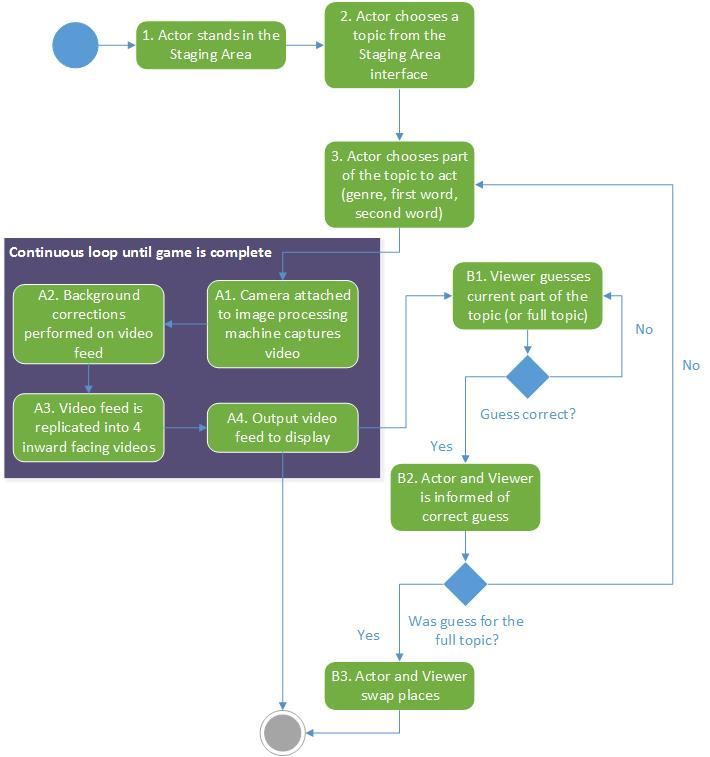
\includegraphics[width=\textwidth]{SystemActivityDiagramImage}

\newpage


\section{Description of Activity Diagram}
\begin{itemize}
	\item [1] Actor is chosen from Viewers by volunteer or at random to be the first actor. Additional system functionality could be added to support choosing the first Actor.
	
	\item [2] Actor is given the choice of a topic from 5 possible topics picked at random by the system and enters their desired phrase to act via the Staging Area interface. \textit{(Staging interface likely to be tablet or similar).}
	
	\item [3] Actor makes a choice on the word of the phrase they wish to act first. This will either be a number for the corresponding word or an option to act the full phrase.
	
	\item [4] The Genre of the phrase being acted (book, film, television show) as well as the current word being acted, is displayed to the Viewer. The Viewer will be in the Viewing area \textit{(where the hologram is being displayed)}.
	
	\item [5] A prompt to begin the image processing loop will be sent. This will turn the camera on (if not already).  
	
	\item \textbf{Image processing loop}

	\subitem [A1] The camera is part of the staging area and points at the actor. The camera will be a peripheral of the image processing machine.
	
	\subitem [A2] The image processing application will perform background subtraction on the camera feed to ensure the background of the video is completely back (remove lighting noise ect.).
	
	\subitem [A3] The video feed will be duplicated into 4 versions of itself and formatted appropriately to work with the Pepper's Ghost Pyramid in the Viewing Area.
	
	\subitem [A4] The video feed is sent to the displaying area.
	
	\item \textbf{Game loop}	
	
	\subitem [B1] The viewer will attempt to guess the current word or full phrase being acted by looking at the hologram. The guess will be made on a tablet (or similar) in the Viewing Area. There may be several tablets available for multiple users.
	
	\subitem [B2] If the guess is correct, then the Viewers and Actor are informed on their respective interface device.
	
	\subitem [B3] If the full phrase has been guessed and the game has finished (reached the full number of rounds). A prompt is sent to the image processing machine to stop the processing loop and the game finishes.
	
	\subitem [B4] If the full phrase has been guessed but the game is not over, the Actor is told to swap places with the Viewer who guessed correctly. The system then returns to the initial state.
	
	
\end{itemize}

\end{document}